% =====================================================================
\section{The Two Equation Flows}
\label{sec:flows}
% =====================================================================

Everything in this guide is organised along two flow diagrams. Every block shows its equations, what goes \textbf{IN}
and what comes \textbf{OUT}; the arrows carry the signals between blocks. Colours: grey = physics (the plant),
orange = the prescribed-performance envelope, magenta = the control law, purple = adaptation, blue = parts that
exist only on the quadcopter.

\begin{figure}[H]
\centering
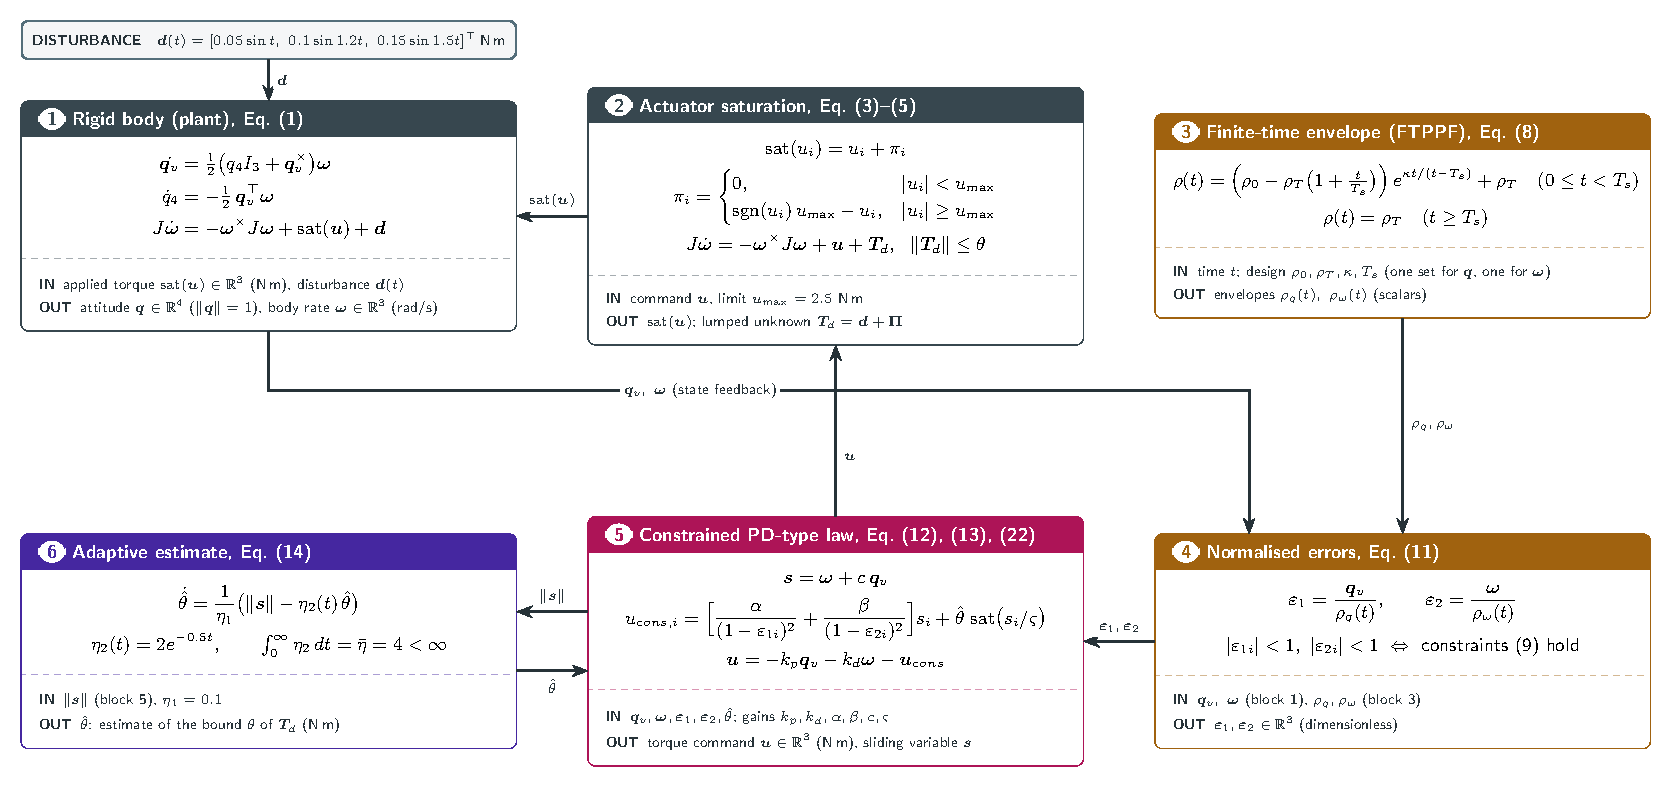
\includegraphics[width=\linewidth]{flow_paper.pdf}
\caption{Flow of the base paper (blocks 1--6). The loop is closed through the state feedback $\qv,\vw$. The disturbance
$\vd(t)$ and the saturation (block 2) are the two things the controller does not know.}
\label{fig:flowpaper}
\end{figure}

\textbf{Reading \cref{fig:flowpaper}.} The plant (block 1) produces the attitude and body rate. The envelope (block 3)
says how large they may be at time $t$; block 4 divides one by the other. The control law (block 5) uses the state,
the normalised errors and the adaptive estimate (block 6) to compute a torque. The actuators can only deliver part of it
(block 2), and that applied torque, together with the disturbance, turns the body again.

\begin{figure}[H]
\centering
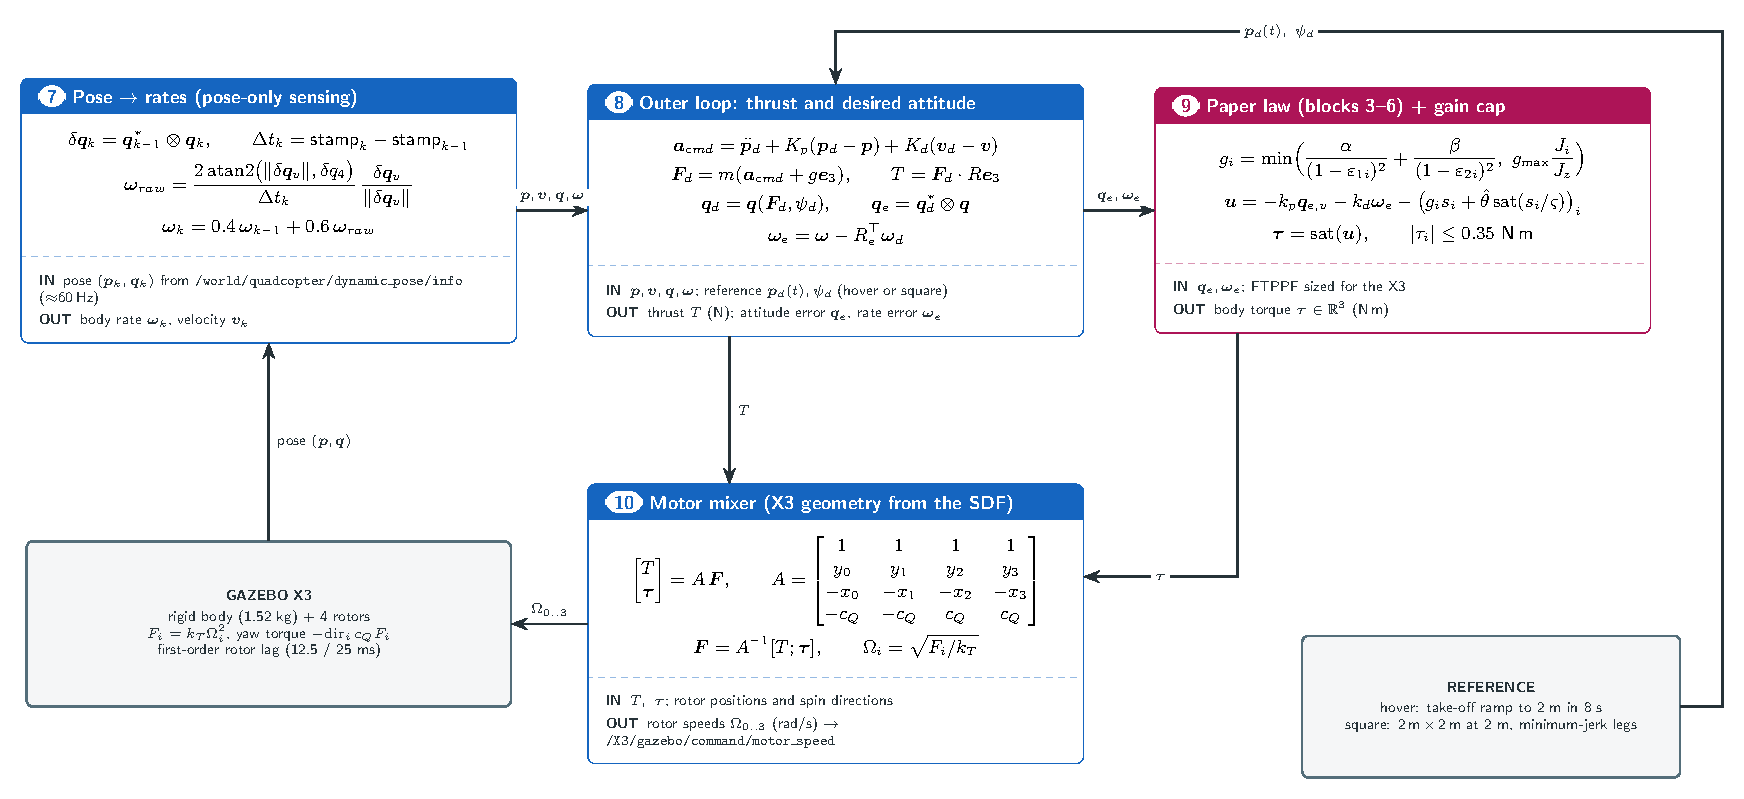
\includegraphics[width=\linewidth]{flow_x3.pdf}
\caption{Flow on the Gazebo X3 quadcopter (blocks 7--10). Blocks 3--6 of \cref{fig:flowpaper} sit inside block 9 unchanged
except for one cap on the barrier gain. Gazebo replaces blocks 1--2: it integrates the real rigid-body and rotor physics.}
\label{fig:flowx3}
\end{figure}

\textbf{Reading \cref{fig:flowx3}.} A quadcopter cannot just turn: it must also hold itself up, and it moves sideways by
tilting. So an \emph{outer} loop (block 8) decides the total thrust and the attitude the drone should have, the paper's
law (block 9) turns the body to that attitude, and the mixer (block 10) splits thrust and torque into four rotor speeds.
Gazebo only publishes the pose, so the body rate is reconstructed from two consecutive quaternions (block 7).

\begin{center}\small
\begin{tabularx}{\linewidth}{@{}c l X l@{}}
\toprule
\textbf{Block} & \textbf{Name} & \textbf{Paper equations} & \textbf{Section}\\
\midrule
1 & Rigid-body attitude dynamics & (1), (2) & \ref{sec:b1}\\
2 & Actuator saturation & (3)--(5) & \ref{sec:b2}\\
3 & Finite-time prescribed performance function & (6)--(8) & \ref{sec:b3}\\
4 & Normalised errors & (9)--(11) & \ref{sec:b4}\\
5 & Constrained PD-type control law & (12), (13), (22) & \ref{sec:b5}\\
6 & Adaptive law & (14) & \ref{sec:b6}\\
-- & Stability proof (Theorem 1) & (15)--(21) & \ref{sec:theorem}\\
7 & Body rate from the pose & -- (ours) & \ref{sec:b7}\\
8 & Outer position loop and desired attitude & -- (ours) & \ref{sec:b8}\\
9 & Paper law on a 60\,Hz loop & (12)--(14) + gain cap & \ref{sec:b9}\\
10 & X3 motor mixer & -- (ours) & \ref{sec:b10}\\
\bottomrule
\end{tabularx}
\end{center}
